%!TEX root = ../thesis.tex

\section{Discussion}
\label{sec:discussion}

% TODO: Say that our properties only restrict machine-mode
% TODO: Say that we meet Alastair's requirements
% TODO: \glspl{ifc}
In section \ref{sec:checking}, a set of IFC properties based on the work in \cite{Ferraiuolo17} has been introduced; we will refer to these properties as the set $ P $.
These properties were model checked in the previous section \ref{sec:results}, the result of which was a set of rules $ R $.
What is the consequence of this?
The formal achievement of this thesis can be summarized as follows:
\begin{quote}
    It can be guaranteed that programs running on the MINRV8 architecture, e.g. \glspl{os}, are \textit{secure} (in the sense of not violating the IFC properties $ P $) if they obey to the rules $ R $.
\end{quote}
But what does \enquote{secure} mean here besides not violating $ P $?
What is the \textit{actual} sense of security that can be guaranteed?

Nothing definite can be said in answer to this question.
However, the canaries these properties have been tested against in section \ref{sec:canaries}, exemplify the class of vulnerabilities that are covered by these properties.

Assessing the results of the approach to formally verify higher level properties of the MINRV8 architecture shall be subject of this section.
We will cover three aspects of our work:
\begin{itemize}
    \item Scope, i.e. what are the limits of our results,
    \item Trustworthiness, i.e. whether our results are sound, and
    \item General observations.
\end{itemize}

\subsection{Scope}
\label{sec:scope}

\subsubsection{Architecture}
\label{sec:discuss-arch}

MINRV8 is meant to be a reasonable abstraction of a real-world RISC-V architecture from a security standpoint.
However, up to this point nothing has been said about the limits of this abstraction.
With every abstraction, there is a small chance that it perfectly matches the concept that has been abstracted in regard to the purpose of the abstraction but in most cases, some corners are cut.
In this section, we will reflect on the limits of the MINRV8 architecture and its implementation.

% TODO: mention that other fields are well modelled
% TODO: mention that we actually don't need all computational instructions
% TODO: mention performance hit of dynamic memory regions

In summary, the MINRV8 architecture knows three groups of instructions (cf. table \ref{tbl:min-arch-instrs}):
\begin{itemize}
    \item Computational instructions such as \minrv{Mov}, \minrv{And}, \minrv{Add}, etc.
    \item Memory instructions \minrv{Load} and \minrv{Store}
    \item System instructions \minrv{Ecall}, \minrv{Mret}, \minrv{Csrrs}, \minrv{Csrrc}
\end{itemize}

A reader, experienced in the field of microcontrollers or computer-architecture in general might wonder why our model does not include:
\begin{enumerate}
    \item Executable memory and a \gls{pc}
    \item Jump or branch instructions
\end{enumerate}

The reason for both of these points lies in the implementation of the model.
In the introduction of the MINRV8 architecture in section \ref{sec:minrv8} we mentioned that the idea of the architecture was tightly coupled to its implementation in nuXmv.
The design of the model had to answer the question: How can a stream of instructions be implemented?
nuXmv allows to think of the following options:
\begin{enumerate}
    \item \label{itm:exmem-frozen}
    Use \smv{FROZENVAR}s to model executable memory - a \smv{FROZENVAR} (frozen variable) is something like a constant in other programming languages but without a fixed value.
    nuXmv chooses the value on the first simulation step but does not change it afterwards.
    This is more efficient than using a plain \smv{VAR} and constraining it to not change, e.g. \smv{TRANS x = next(x);}.
    \item \label{itm:exmem-var}
    Use \smv{VAR}s to model executable memory.
    In practice, this would mean that the memory of the implementation as described in section \ref{sec:model-implementation} would be much larger than the current 4 bytes.
    \item \label{itm:exmem-ivar}
    Finally, use \smv{IVAR}s to model the stream of instruction.
    This is the option we decided to go for as described in section \ref{sec:model-implementation}.
    Using input variables means that there is no model of executable memory.
    Instead, the input variables provided to the implementation model a stream of a fully decoded instruction on each transition of the simulated model.
    As such, the architecture does not need to worry \textit{where} these instructions come from.
\end{enumerate}

The decision towards using input variables as a model of the stream of instructions was made because of two reasons:
\begin{enumerate*}[label=\alph*)]
    \item in the prototyping phase of the model, it was quickly found out that using input variables led to significant boosts in performance, and
    \item using input variable simplified the implementation significantly.
\end{enumerate*}
Having used purely either frozen variables or variables would have increased the size of the state space to be traversed by nuXmv and would have introduced the necessity to implement instruction decoding increasing the complexity of the transition relation.
Furthermore, it would not have allowed for unbounded model checking of the architecture since the size of programs to be taken into consideration would have been bounded by the size of executable memory.

Yet, using input variables also has some downsides.
First and foremost, using input variables means that it is pointless to model a \gls{pc} or anything address related like return addresses, a dedicated \gls{lr} or \glspl{csr} such as \gls{mtvec} as without a model of executable memory there is nothing addresses could point to.
Instead, instructions will simply magically appear on each cycle of the processor model.
This means that the simulation is inaccurate in this regard which in itself is not a problem.
The model is supposed to be an abstraction.
Since it was decided to use input variables over a model of the \gls{mtvec} register and a \gls{pc}, the question now arises how accurately the implementation of the MINRV8 architecture is capable to simulate real architectures.
In a nutshell, the use of input variables over (frozen) variables introduces a certain sense of non-determinism to the model of the MINRV8 architecture when it comes to handling interrupts and exceptions.

\begin{figure}
    \centering
    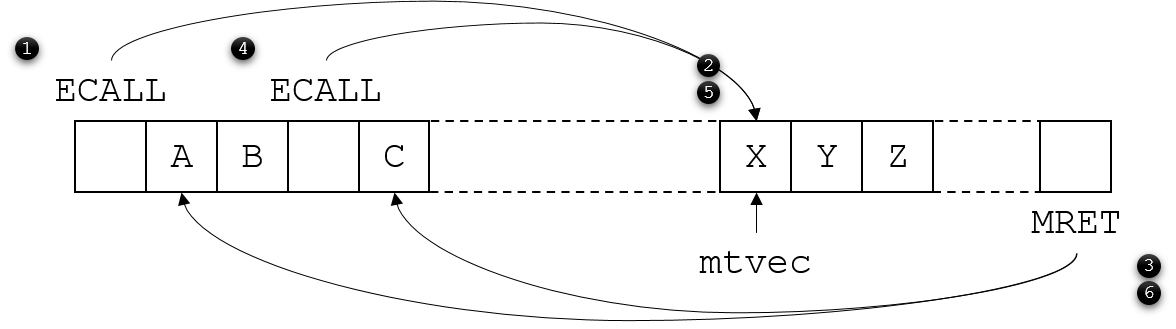
\includegraphics[width=0.7\textwidth]{figures/interrupt-flow.png}
    \caption{Program flow involving interrupts}
    \label{fig:interrupt-flow}
\end{figure}

Consider an example memory layout for the RISC-V architecture as depicted in figure \ref{fig:interrupt-flow} where code is executed from left to right starting with an \minrv{Ecall} instruction.
Executing this instruction triggers a shift in control to machine-mode which jumps to address \minrv{X} pointed to by the \gls{mtvec} register.
Then, the instructions at addresses \minrv{X} to \minrv{Z} and subsequent ones are executed until finally, a \minrv{Mret} instruction is read an executed which triggers a jump to address \minrv{A}.
Two instructions later, another \minrv{Ecall} instruction is executed, etc.
We would expect the order of instructions to be executed to look like:

\begin{enumerate}
    \item First environment call: \lstinline[language=minrv8,mathescape=true]{Ecall, Load, Add, Store, $\dots$, Mret}
    \item Return: \lstinline[language=minrv8,mathescape=true]{Load, Mov}
    \item Second environment call: \lstinline[language=minrv8,mathescape=true]{Ecall, Load, Add, Store, $\dots$, Mret}
    \item Second return: \lstinline[language=minrv8,mathescape=true]{Slt, $\dots$}
\end{enumerate}
Where \minrv{Load, Add, Store} are the instructions located at addresses \minrv{X} to \minrv{Z} and \minrv{Load, Mov, Slt} the instructions located at addresses \minrv{A}, \minrv{B} and \minrv{C} respectively.

As input variables can not be constrained in nuXmv, there is no way to model that the instructions being executed on a trap always are equal, i.e. a valid stream of instructions as a sequence of input variable valuations to the model might be:
\begin{enumerate}
    \item First environment call: \lstinline[language=minrv8,mathescape=true]{Ecall, Load, Add, Store, $\dots$, Mret}
    \item Return: \lstinline[language=minrv8,mathescape=true]{Load, Mov}
    \item Second environment call: \lstinline[language=minrv8,mathescape=true]{Ecall, And, Sra, $\dots$, Mret}
    \item Second return: \lstinline[language=minrv8,mathescape=true]{Slt, $\dots$}
\end{enumerate}

Such a stream of instructions is not realistic without some program modifying the code located at \gls{mtvec} and as such \enquote{shouldn't} be considered when checking the IFC properties.
One would expect to find the same code after an \minrv{Ecall} instruction being executed since in both cases, an architecture would jump to the respective interrupt handler.
However, there of course also exists a sequence of input variable valuations that exactly match a \enquote{real} stream of instructions where the instructions executed after an environment call coincide.

This illustrates one example for why the implementation of the MINRV8 \textit{abstracts} from real architectures.
In regard to program flow on traps, it can be expected that the model accurately comprises all expected streams of instructions but also includes many more one would naturally consider to be unrealistic.

The second concept, the abstract implementation of the MINRV8 architecture is missing are jump an branch instructions.
They are missing for the exact same reasons as described in the previous paragraphs.
Since the implementation does not support executable memory and as such does not support addresses, jumps and branches are pointless instructions.
This, however, does not turn out to be a fundamental problem.
In principle, jump and branch instructions in real systems are security relevant since they are used to perform function calls and returns and implement loops or conditional statements.
% TODO: \gls{rop}
In practice though, jumps and branches usually are security relevant since they are targeted by adversarial programs trying to manipulate jump addresses to launch ROP attacks.
ROP attacks are only effective because they jump to locations where critical code is located.
It does not matter whether the critical code is executed without the intervention of some malicious program or whether some malicious program tricks privileged code into executing said critical code - in practice, the former case simply occurs rarely.
The concept of jumps being influenced by some malicious program is, however, captured in approach: both properties \ref{itm:prop-mem-i} and \ref{itm:prop-csr-i}, i.e. the integrity of memory- and \gls{csr}- related instruction, ensure that certain instructions may not be influenced by user-mode.
There is no reason to assume that user-mode would control jumps and branches by fundamentally different flows of information than memory- and \gls{csr}-related instructions, i.e. jump related vulnerabilities are covered in principle.

Additionally, our implementation might not be able to model programs including jumps and branches but the set of programs considered by nuXmv does include those where jumps have been linearized\footnote{%
    This is similar to function inlining supported by many compilers.
}.
Consider figure \ref{fig:jump-inlining} where in the upper half depicts an ordinary program, being executed from left to right and including jump instructions.
Jump linearization here means that for any such program there also exists another (potentially infinite) program where no jumps occur but the same instructions besides jumps are being executed.
The respective counterpart to the program in the upper half is depicted in the lower half of figure \ref{fig:jump-inlining}.
The sequence of states generated by the linearized programs is equal to the sequence of states of the non-linearized program modulo \gls{pc} values - which is not modelled in nuXmv anyways.

\begin{figure}
    \centering
    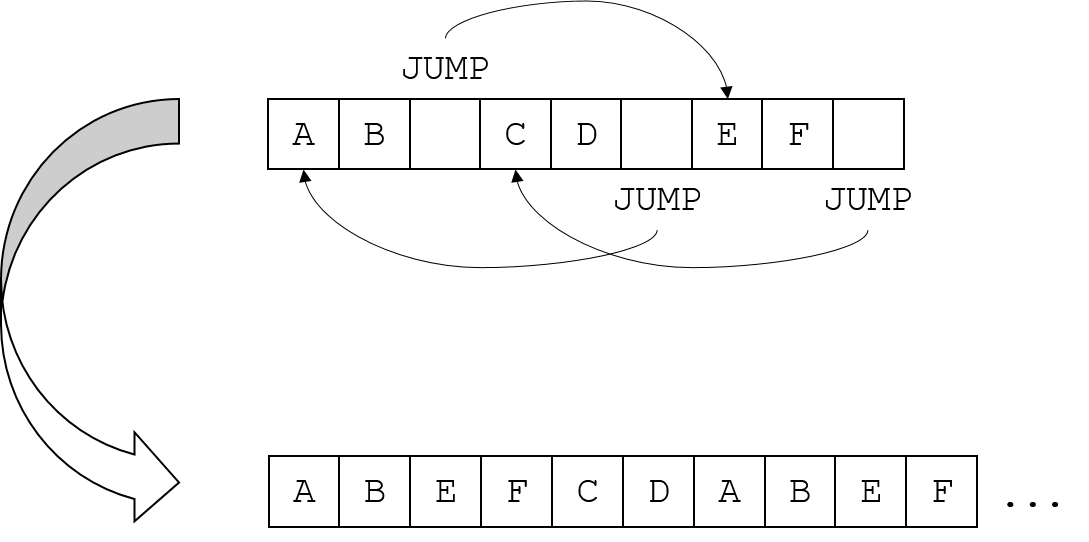
\includegraphics[width=0.7\textwidth]{figures/jump-free-programs.png}
    \caption{Jump linearization}
    \label{fig:jump-inlining}
\end{figure}

\paragraph{Summary}

% TODO: My implementation of the stream of instructions is an over-abstraction

Starting with the premise of this thesis, it was always clear that the MINRV8 architecture is a simplification.
This, though, is not a problem since by focusing on the very core, security related instructions allowed us to implement a tractable and small model in nuXmv.
If one would add jump and branch instructions to the MINRV8 architecture, it'd be comparable to actual RISC-V architectures.
From this point of view, it is not a problem to apply the results of the verification process, i.e. the set of assumptions, to the RISC-V architecture.

The implementation of the MINRV8 architecture abstracted from real-world architectures in two main points:
\begin{enumerate}
    \item nuXmv does not guarantee stable behavior on \minrv{Ecall} instructions; this introduces a sense of non-determinism for which there are more programs considered by nuXmv than could actually be run on the MINRV8 architecture.
    This is not problematic because overabstracting the space of all programs $ P $ still leaves nuXmv considering all programs in $ P $.
    \item The implementation does not support jump or branch instructions.
    This is not problematic because
    \begin{enumerate*}[label=\alph*)]
        \item flows of information relevant to jump and branch instructions are still covered by the integrity properties \ref{itm:prop-mem-i} and \ref{itm:prop-csr-i} and
        \item programs including jumps can be linearized; such programs \textit{are} considered by nuXmv.
    \end{enumerate*}
\end{enumerate}

This leaves us with good reasons to assume that programs considered by nuXmv, i.e. the set of programs quantified over when running proofs, is sufficiently close to the set of \enquote{real} programs of the MINRV8 architecture including jumps and branches.
% TODO: Future work?

\subsubsection{Assumptions}

% TODO: Mention these goals in introduction/background

The goal we had in mind when phrasing the assumptions which ultimately established the correctness of the information flow properties was for them to be realistic.
This goal includes:
\begin{enumerate}
    \item \label{itm:assumptions-non-trivial}
    The assumptions must be non-trivial, i.e. they must not be contradictory and must not trivially entail the information flow properties to be verified,
    \item \label{itm:assumptions-machine-mode}
    the assumptions must only constrain machine-mode,
    \item \label{itm:assumptions-verifiable}
    the assumptions must be decidable and verifiable.
\end{enumerate}

The reasoning behind point \ref{itm:assumptions-non-trivial} is straight-forward:
Trying to prove \enquote{$ \text{false} \Rightarrow \text{properties} $} or \enquote{$ \text{properties} \Rightarrow \text{properties} $} is pointless.
Although we can't give formal proofs that neither is the case, we have good reasons to believe it.
Recall that we were able to prove that \enquote{$ \text{assumptions} \Leftrightarrow \text{properties} $}.
In this case, the assumptions can only be contradictory if the properties are as well which we think, they are obviously not.
On the other hand, recall that in section \ref{sec:canaries} we were able to make changes to the architecture such that \enquote{$ \neg(\text{assumptions} \Rightarrow \text{properties}) $} held.
This indicates clearly that the assumption actually express something meaningful and do not trivially entail the information flow properties.

Point \ref{itm:assumptions-machine-mode} also is met by the assumptions introduced in section \ref{sec:assumptions}.
Whenever it is said that certain instructions must not be executed under certain circumstances, these formulas are guarded by the antecedent \smv{priv ->}.
Additionally, all other assumptions only constrain state transitions that are under control of machine-mode only, such as changes to \glspl{csr} or state before machine-mode hands back control to user-mode.
All in all, this point does not need to be discussed extensively.
However, it was raised nonetheless because it is important to note that the assumptions introduced as a result of this thesis fit in the threat model as discussed in section \ref{sec:threat-model}.
Recall, that in context of this thesis it is assumed that user-mode is adversarial to machine-mode and compromised completely.
Constraining user-mode in the assumptions therefore would have contradicted this threat model.

Lastly, the most critical point is point \ref{itm:assumptions-verifiable}.
Ideally, the assumptions established in context of this thesis would serve as a verification target for \glspl{os} or compilers.
If one was to write a collection of interrupt handlers for an \gls{os}, one might want to check that all 8 assumptions are implemented by these.
This would grant the absence of information flow related bugs in context of the information flow properties as proposed in section \ref{sec:checking}.
This, however, presupposes that it is actually possible to verify programs against these properties.
As part of this thesis, we cannot give guarantees on the feasibility of this undertaking.
Yet, we tried to allow for it.
Meeting point \ref{itm:assumptions-machine-mode} is one step in the right direction.
However, how these simplified properties might be transferred to real-world system is an open question.
The problems behind this are illustrated by the \smv{SP_BANK} assumption introduced parallel to the SYSRET vulnerability in section \ref{sec:sysret}.
There are two aspects of the first part of this assumption which are noteworthy.
The relevant part of the \smv{SP_BANK} assumption is given in snippet \ref{snpt:sp-bank-p1}.

\begin{figure}
    \begin{lstlisting}[
        language=smv,
        caption={First part of the assumption \lstinline{SP_BANK}},
        label={snpt:sp-bank-p1}
    ]
        G (!priv & X priv -> X ( (*\label{ln:sp-call-priv}*)
            (priv -> !(op in { PUSH, POP }))
            U ((op = MRET & MPP = 0b_0) | sp[sp_sel] < $REGION0_SIZE (*\label{ln:sp-call-mret}*)
                ? !pmpcfg0.write & !pmpcfg0.read
                : !pmpcfg1.write & !pmpcfg1.read)
        )) &
    \end{lstlisting}
\end{figure}

Whilst working on this assumption, we found that the specific implementation of two \textit{ideas} was critical to the presence of the SYSRET vulnerability, both:
\begin{enumerate}
    \item \label{itm:no-sysret-priv}
    replacing the expression \smv{!priv & X priv} in line \ref{ln:sp-call-priv} by \smv{(op = ECALL) | (bool(MIE) & bool(MEIP))} which is the actual condition under which a trap is taken and
    \item \label{itm:no-sysret-mret}
    omitting the expression \smv{(op = MRET & MPP = 0b_0)} in line \ref{ln:sp-call-mret}
\end{enumerate}
led to nuXmv not finding the SYSRET vulnerability.
Why is that?

The first part of the \smv{SP_BANK} assumption states: \enquote{Whenever there is a switch from user- to machine-mode, latter can only use the \minrv{Push} or \minrv{Pop} instructions after having returned to user-mode or having ensured that the stack-pointer is safe}.
If the antecedent of this assumption would have been replaced by: \enquote{Whenever a trap is taken, \dots}, i.e. by \smv{(op = ECALL) | (bool(MIE) & bool(MEIP))}, the consequent would also have applied to cases where a trap was taken from machine-mode to machine-mode\footnote{
    Furthermore, it is noteworthy that the antecedent in the original assumption resembles a more result-driven approach to phrasing properties, i.e. talk about \textit{what} is happening, whereas the alternative disucssed here resembles a more architecture-driven approach, i.e. talk about \textit{when} things are happening.
    The discussion, which of these approaches should be preferred is a topic on its own.
    In this thesis, we used both approaches but tried to stick to the result-driven approach whenever possible to keep the assumptions concise.
    In certain situations, however, it was more practical to go for the architecture-driven approach.
}.
Such a trap is necessary to interrupt machine-mode from properly returning to user-mode while already having set the stack-pointer back to user-mode.
The consequent also applying to traps from machine- to machine-mode in context of the MINRV8 architecture boils down to machine-mode ensuring that the proper stack-pointer is setup correctly on \textit{all} traps rendering the SYSRET vulnerability impossible.
For example, the \glspl{os} being affected by the SYSRET vulnerability clearly did not set the stack-pointer on \textit{all} execution paths of the trap handler for the general protection fault.

The condition \smv{(op = MRET & MPP = 0b_0)} on the right-hand side of the \smv{U}-expression in line \ref{ln:sp-call-mret} equals telling machine-mode: \enquote{You can forget about not using the \minrv{Push} and \minrv{Pop} instructions after you have \textit{attempted} to return control to user-mode}.
For the same reasons as stated above, this part is critical.
Leaving this expression out would equal machine-mode having state persistent over user-mode-calls and -returns to and from machine-mode, by which machine-mode memorizes whether it has set the stack-pointer to user-mode or to machine-mode.
With such a mechanism in place, machine-mode could not be fooled into using the user-mode stack-pointer on any trap handler since it would first check this state.

These two examples stress that the precise phrasing of the assumptions is highly critical for both how realistic the assumptions are and how well they might be suited to serve as target for verification of actual code-bases.
While it would be sufficient to find a stronger precondition for these assumptions in existing code-bases, it is non-trivial whether such preconditions are easy to find or whether the assumptions might be rephrased such that they still grant the absence of information flow related bugs but are easier to verify in programs.
This topic, though, can't be handled as part of this thesis leading to future work.

\subsection{Trustworthiness}
\label{sec:trustworthiness}

Verification processes must not be arbitrary.
The core of verification is to enhance the trust in a given system.
For trust to arise, it is mandatory for the process itself to be trustworthy.

But what does \textit{trustworthy} mean?
Here, we will skip the aspect of technical soundness of this thesis, i.e. the question of whether the work presented in this thesis is without errors.
In consequence, the degree of trustworthiness is determined by whether the results of the verification process actually enhance the confidence in the correctness of the MINRV8 architecture, i.e. rather than asking whether we did what we did right, we ask: did we do the \textit{right} thing?
\citeauthor{Piano} expressed this sense of trustworthiness in his blog post \citetitle{Piano} as:
\textcquote{Piano}{\textins{I}t is extremely difficult to argue convincingly that a verification result is correct. By \enquote{correct} I mean not only \enquote{mathematically sound} but also \enquote{the result is faithful to the intent of the verification effort.}}

A possible issue with verification is to make circular arguments (an example for this will be given in section \ref{sec:related-work}).
Verification engineers do not start their work out of nowhere.
They usually have a feel for what they attempt to verify and have some vulnerabilities in mind they try to tackle.
If the actual work of modeling a prototype and implementing a verification procedure is influenced by this too strongly, one might object:
\enquote{You were able to find vulnerability \textit{X} only because you knew that it was there. Your procedure is nothing but an abstracted simulation of known issues.}

This also leads to another concern:
As with most programming, the verification process will tackle what is aimed for in some more general sense, i.e. when aiming to verify systems against certain bugs these are usually generalized to classes of related vulnerabilities.
But with such an approach, one can never be sure that there is no other class of vulnerabilities that was missed.
In other words: Does the verification procedure have blind spots?

It shall now be subject to investigate whether our work is touched by aforementioned two issues.

First, we will investigate whether our thesis has made a circular argument.
Recall the steps that have been taken to verify the MINRV8 architecture against the information flow properties:
% TODO: Cite respective sections
\begin{enumerate}
    \item \label{itm:step-minrv}
    Specify the MINRV8 architecture based on RISC-V
    \item \label{itm:step-semantics}
    Define information flow semantics for the instructions available on MINRV8
    \item \label{itm:step-properties}
    Use fields not being propagated in the information flow semantics and some intuition to state information flow properties
    \item \label{itm:step-loop}
    Enter a proof-refine-loop until a fixpoint has been reached
    \item \label{itm:step-canaries}
    Test the model by subjecting it to vulnerabilities
\end{enumerate}

We find that steps \ref{itm:step-semantics} to \ref{itm:step-loop} are well founded by both theory and intuition and do obviously not face the risk of making a circular argument.
This, however, is less obvious for steps \ref{itm:step-minrv} and \ref{itm:step-canaries}.
In both cases, the selection of RISC-V features and instruction to include or vulnerabilities to test respectively can be doubted.

The work on this thesis was indeed influenced by the canaries the model was ultimately tested against and vice versa: the selection of vulnerabilities to test the model against was based on the features implemented in it.
Despite the ciruclar character of these two steps, we find that this is not an issue.
Steps \ref{itm:step-minrv} and \ref{itm:step-canaries} must be understood as a prototype of a verification procedure proposed in this thesis which is given by steps \ref{itm:step-semantics} to \ref{itm:step-loop}.
Having the setup to test these steps in being derived via a methodology that is circular to some degree does not make the procedure itself circular.
The opposite is the case:
We find that the definition of information flow semantic, information flow control properties and the proof-refine-loop are all well founded and comprehensible, i.e. follow some intuition which could make one have more trust in the given system.

On the other hand, we must admit that it is unknown whether there are blind spots to the verification procedure or more precisely: to the information flow control properties.
We managed to show that these properties are not meaningless since they are able to detect both the SYSRET and the cache poisoning vulnerability.
But it is unclear
\begin{enumerate*}[label=\alph*)]
    \item which class of bugs or vulnerabilities can be detected by this procedure and
    \item whether this class covers \textit{all} vulnerabilities in the sense of \citeauthor{Piano}, i.e. \textcquote{Piano}{the result is faithful to the intent of the verification effort.}
\end{enumerate*}
We mark this problem as future work.

\subsection{General Observations}
\label{sec:discuss-observations}

\subsubsection{Abstract Model}

You as a reader might have wondered, why we decided to concretely model all flow of information through the model of the MINRV8 architecture and indeed: In the very scope of this thesis, the actual content of registers is not mandatory.
It does play a role when memory is indexed, but one could probably get away with non-deterministically choosing a memory location to be targeted by loads and stores.

There are two reasons for why this decision was made.
Firstly, since the work of \citeauthor{Ferraiuolo17} \cite{Ferraiuolo17} was adopted more or less directly where the authors did rely on precise values to track\footnote{%
    This is due to the fact that \gls{hdl} code is annotated.
    Or in other words: the authors did not have a chance to not track precise values.
} and performance of nuXmv did not mandate to shrink the model, it initially was decided to model values in the MINRV8 architecture.

However, secondly, working with concrete values has two benefits which might become important in future work.
\begin{enumerate}
    \item If the model ever was to be extended by jumps and branches, deterministic addresses are needed to model static code in executable memory.
    If not only loads and stores but also jumps and branches would use non-deterministic mechanisms to determine target addresses, modelling executable memory (cf. sec. \ref{sec:discuss-arch}) and for example interrupt handlers located in this very memory would be pointless to begin with.
    \item Deterministic values lead to counter-examples being easier to interpret.
\end{enumerate}

With these two reasons at hand and the overall goal of this thesis to implement a prototype for a methodology to verify \glspl{isa}, we find that having used concrete values improves on the significance of our results.

\subsubsection{Per-Bit Information Flow Tracking}

Another issue, a reader might have stumbled upon is that in section \ref{sec:results} it was mentioned that counter-examples never involved spurious flows of information where the bit-wise labels of values in the architecture was mandatory.
In other words: for this thesis, tracking only one bit for confidentiality and one bit for integrity for each register and memory address would suffice.
Initially, it was decided to track labels bit-wise because \begin{enumerate*}[label=\alph*)]
    \item we followed the approach of \citeauthor{Ferraiuolo17} \cite{Ferraiuolo17} which tracked information flow bit-wise as well,
    \item again, performance was sufficient to allow for it, and
    \item we couldn't have been sure prima facie non-bit-wise tracking of information would suffice.
\end{enumerate*}

Additionally, it can also be seen that computational instructions never played a major role in any counter-example.
These results suggest that in future work, if the model ever was to be expanded to a more accurate model of RISC-V and/or to a higher machine-word width and performance problems then are encountered, one could abstract the information flow tracking labels from bit- to word-wise labels or one could remove instructions that only alter data but do not add \enquote{new} ways for information to flow.
E.g. the \minrv{Add} instruction - from a pure standpoint of \textit{where} information flows - adds nothing in comparison to the \minrv{Mov} instruction.
The former option only shrinks the state space by a linear factor whereas a register-width increases it exponentially - nevertheless this might matter.

The gist of these findings is:
Whereas in the work of \citeauthor{Ferraiuolo17} \cite{Ferraiuolo17} tracking of each and every bit for a given system was crucial because the authors \textit{could not choose where bugs occur}, it seems that in our more-high level approach for every bug \enquote{imaginable}, there is a very simple trace illustrating it: nuXmv is able to choose where a bug occurs since it quantifies over programs as opposed to the work of \citeauthor{Ferraiuolo17} where the program of interest is fixed.

It must be part of future work to investigate whether reducing the instruction set to instructions such as \minrv{Mov}, \minrv{Load}, \minrv{Store} also is possible when executable memory is modelled (cf. sec. \ref{sec:discuss-arch}).
In this case, an attacker might need to rely on crafting specific payloads to trigger a vulnerability in some static code in executable memory\footnote{%
    It also is imaginable that the attacker would not need to rely on crafting specific payloads because for every scenario where such a payload would be needed, there also is a scenario in which a more simple payload does suffice since nuXmv still quantifies over the static parts of the code.
    However, we don't find that a decision regarding this question can be made here.
}.
